% Options for packages loaded elsewhere
\PassOptionsToPackage{unicode}{hyperref}
\PassOptionsToPackage{hyphens}{url}
\PassOptionsToPackage{dvipsnames,svgnames,x11names}{xcolor}
%
\documentclass[
  letterpaper,
  DIV=11,
  numbers=noendperiod]{scrartcl}

\usepackage{amsmath,amssymb}
\usepackage{iftex}
\ifPDFTeX
  \usepackage[T1]{fontenc}
  \usepackage[utf8]{inputenc}
  \usepackage{textcomp} % provide euro and other symbols
\else % if luatex or xetex
  \usepackage{unicode-math}
  \defaultfontfeatures{Scale=MatchLowercase}
  \defaultfontfeatures[\rmfamily]{Ligatures=TeX,Scale=1}
\fi
\usepackage{lmodern}
\ifPDFTeX\else  
    % xetex/luatex font selection
    \setmainfont[]{Times New Roman}
\fi
% Use upquote if available, for straight quotes in verbatim environments
\IfFileExists{upquote.sty}{\usepackage{upquote}}{}
\IfFileExists{microtype.sty}{% use microtype if available
  \usepackage[]{microtype}
  \UseMicrotypeSet[protrusion]{basicmath} % disable protrusion for tt fonts
}{}
\makeatletter
\@ifundefined{KOMAClassName}{% if non-KOMA class
  \IfFileExists{parskip.sty}{%
    \usepackage{parskip}
  }{% else
    \setlength{\parindent}{0pt}
    \setlength{\parskip}{6pt plus 2pt minus 1pt}}
}{% if KOMA class
  \KOMAoptions{parskip=half}}
\makeatother
\usepackage{xcolor}
\usepackage[lmargin=2cm,rmargin=2cm,tmargin=1.5cm]{geometry}
\setlength{\emergencystretch}{3em} % prevent overfull lines
\setcounter{secnumdepth}{5}
% Make \paragraph and \subparagraph free-standing
\makeatletter
\ifx\paragraph\undefined\else
  \let\oldparagraph\paragraph
  \renewcommand{\paragraph}{
    \@ifstar
      \xxxParagraphStar
      \xxxParagraphNoStar
  }
  \newcommand{\xxxParagraphStar}[1]{\oldparagraph*{#1}\mbox{}}
  \newcommand{\xxxParagraphNoStar}[1]{\oldparagraph{#1}\mbox{}}
\fi
\ifx\subparagraph\undefined\else
  \let\oldsubparagraph\subparagraph
  \renewcommand{\subparagraph}{
    \@ifstar
      \xxxSubParagraphStar
      \xxxSubParagraphNoStar
  }
  \newcommand{\xxxSubParagraphStar}[1]{\oldsubparagraph*{#1}\mbox{}}
  \newcommand{\xxxSubParagraphNoStar}[1]{\oldsubparagraph{#1}\mbox{}}
\fi
\makeatother

\usepackage{color}
\usepackage{fancyvrb}
\newcommand{\VerbBar}{|}
\newcommand{\VERB}{\Verb[commandchars=\\\{\}]}
\DefineVerbatimEnvironment{Highlighting}{Verbatim}{commandchars=\\\{\}}
% Add ',fontsize=\small' for more characters per line
\usepackage{framed}
\definecolor{shadecolor}{RGB}{241,243,245}
\newenvironment{Shaded}{\begin{snugshade}}{\end{snugshade}}
\newcommand{\AlertTok}[1]{\textcolor[rgb]{0.68,0.00,0.00}{#1}}
\newcommand{\AnnotationTok}[1]{\textcolor[rgb]{0.37,0.37,0.37}{#1}}
\newcommand{\AttributeTok}[1]{\textcolor[rgb]{0.40,0.45,0.13}{#1}}
\newcommand{\BaseNTok}[1]{\textcolor[rgb]{0.68,0.00,0.00}{#1}}
\newcommand{\BuiltInTok}[1]{\textcolor[rgb]{0.00,0.23,0.31}{#1}}
\newcommand{\CharTok}[1]{\textcolor[rgb]{0.13,0.47,0.30}{#1}}
\newcommand{\CommentTok}[1]{\textcolor[rgb]{0.37,0.37,0.37}{#1}}
\newcommand{\CommentVarTok}[1]{\textcolor[rgb]{0.37,0.37,0.37}{\textit{#1}}}
\newcommand{\ConstantTok}[1]{\textcolor[rgb]{0.56,0.35,0.01}{#1}}
\newcommand{\ControlFlowTok}[1]{\textcolor[rgb]{0.00,0.23,0.31}{\textbf{#1}}}
\newcommand{\DataTypeTok}[1]{\textcolor[rgb]{0.68,0.00,0.00}{#1}}
\newcommand{\DecValTok}[1]{\textcolor[rgb]{0.68,0.00,0.00}{#1}}
\newcommand{\DocumentationTok}[1]{\textcolor[rgb]{0.37,0.37,0.37}{\textit{#1}}}
\newcommand{\ErrorTok}[1]{\textcolor[rgb]{0.68,0.00,0.00}{#1}}
\newcommand{\ExtensionTok}[1]{\textcolor[rgb]{0.00,0.23,0.31}{#1}}
\newcommand{\FloatTok}[1]{\textcolor[rgb]{0.68,0.00,0.00}{#1}}
\newcommand{\FunctionTok}[1]{\textcolor[rgb]{0.28,0.35,0.67}{#1}}
\newcommand{\ImportTok}[1]{\textcolor[rgb]{0.00,0.46,0.62}{#1}}
\newcommand{\InformationTok}[1]{\textcolor[rgb]{0.37,0.37,0.37}{#1}}
\newcommand{\KeywordTok}[1]{\textcolor[rgb]{0.00,0.23,0.31}{\textbf{#1}}}
\newcommand{\NormalTok}[1]{\textcolor[rgb]{0.00,0.23,0.31}{#1}}
\newcommand{\OperatorTok}[1]{\textcolor[rgb]{0.37,0.37,0.37}{#1}}
\newcommand{\OtherTok}[1]{\textcolor[rgb]{0.00,0.23,0.31}{#1}}
\newcommand{\PreprocessorTok}[1]{\textcolor[rgb]{0.68,0.00,0.00}{#1}}
\newcommand{\RegionMarkerTok}[1]{\textcolor[rgb]{0.00,0.23,0.31}{#1}}
\newcommand{\SpecialCharTok}[1]{\textcolor[rgb]{0.37,0.37,0.37}{#1}}
\newcommand{\SpecialStringTok}[1]{\textcolor[rgb]{0.13,0.47,0.30}{#1}}
\newcommand{\StringTok}[1]{\textcolor[rgb]{0.13,0.47,0.30}{#1}}
\newcommand{\VariableTok}[1]{\textcolor[rgb]{0.07,0.07,0.07}{#1}}
\newcommand{\VerbatimStringTok}[1]{\textcolor[rgb]{0.13,0.47,0.30}{#1}}
\newcommand{\WarningTok}[1]{\textcolor[rgb]{0.37,0.37,0.37}{\textit{#1}}}

\providecommand{\tightlist}{%
  \setlength{\itemsep}{0pt}\setlength{\parskip}{0pt}}\usepackage{longtable,booktabs,array}
\usepackage{calc} % for calculating minipage widths
% Correct order of tables after \paragraph or \subparagraph
\usepackage{etoolbox}
\makeatletter
\patchcmd\longtable{\par}{\if@noskipsec\mbox{}\fi\par}{}{}
\makeatother
% Allow footnotes in longtable head/foot
\IfFileExists{footnotehyper.sty}{\usepackage{footnotehyper}}{\usepackage{footnote}}
\makesavenoteenv{longtable}
\usepackage{graphicx}
\makeatletter
\def\maxwidth{\ifdim\Gin@nat@width>\linewidth\linewidth\else\Gin@nat@width\fi}
\def\maxheight{\ifdim\Gin@nat@height>\textheight\textheight\else\Gin@nat@height\fi}
\makeatother
% Scale images if necessary, so that they will not overflow the page
% margins by default, and it is still possible to overwrite the defaults
% using explicit options in \includegraphics[width, height, ...]{}
\setkeys{Gin}{width=\maxwidth,height=\maxheight,keepaspectratio}
% Set default figure placement to htbp
\makeatletter
\def\fps@figure{htbp}
\makeatother

\KOMAoption{captions}{tableheading}
\makeatletter
\@ifpackageloaded{tcolorbox}{}{\usepackage[skins,breakable]{tcolorbox}}
\@ifpackageloaded{fontawesome5}{}{\usepackage{fontawesome5}}
\definecolor{quarto-callout-color}{HTML}{909090}
\definecolor{quarto-callout-note-color}{HTML}{0758E5}
\definecolor{quarto-callout-important-color}{HTML}{CC1914}
\definecolor{quarto-callout-warning-color}{HTML}{EB9113}
\definecolor{quarto-callout-tip-color}{HTML}{00A047}
\definecolor{quarto-callout-caution-color}{HTML}{FC5300}
\definecolor{quarto-callout-color-frame}{HTML}{acacac}
\definecolor{quarto-callout-note-color-frame}{HTML}{4582ec}
\definecolor{quarto-callout-important-color-frame}{HTML}{d9534f}
\definecolor{quarto-callout-warning-color-frame}{HTML}{f0ad4e}
\definecolor{quarto-callout-tip-color-frame}{HTML}{02b875}
\definecolor{quarto-callout-caution-color-frame}{HTML}{fd7e14}
\makeatother
\makeatletter
\@ifpackageloaded{caption}{}{\usepackage{caption}}
\AtBeginDocument{%
\ifdefined\contentsname
  \renewcommand*\contentsname{Table of contents}
\else
  \newcommand\contentsname{Table of contents}
\fi
\ifdefined\listfigurename
  \renewcommand*\listfigurename{List of Figures}
\else
  \newcommand\listfigurename{List of Figures}
\fi
\ifdefined\listtablename
  \renewcommand*\listtablename{List of Tables}
\else
  \newcommand\listtablename{List of Tables}
\fi
\ifdefined\figurename
  \renewcommand*\figurename{Figure}
\else
  \newcommand\figurename{Figure}
\fi
\ifdefined\tablename
  \renewcommand*\tablename{Table}
\else
  \newcommand\tablename{Table}
\fi
}
\@ifpackageloaded{float}{}{\usepackage{float}}
\floatstyle{ruled}
\@ifundefined{c@chapter}{\newfloat{codelisting}{h}{lop}}{\newfloat{codelisting}{h}{lop}[chapter]}
\floatname{codelisting}{Listing}
\newcommand*\listoflistings{\listof{codelisting}{List of Listings}}
\makeatother
\makeatletter
\makeatother
\makeatletter
\@ifpackageloaded{caption}{}{\usepackage{caption}}
\@ifpackageloaded{subcaption}{}{\usepackage{subcaption}}
\makeatother
\makeatletter
\@ifpackageloaded{tikz}{}{\usepackage{tikz}}
\makeatother
        \newcommand*\circled[1]{\tikz[baseline=(char.base)]{
          \node[shape=circle,draw,inner sep=1pt] (char) {{\scriptsize#1}};}}  
                  

\ifLuaTeX
  \usepackage{selnolig}  % disable illegal ligatures
\fi
\usepackage{bookmark}

\IfFileExists{xurl.sty}{\usepackage{xurl}}{} % add URL line breaks if available
\urlstyle{same} % disable monospaced font for URLs
\hypersetup{
  pdftitle={Statistics Review},
  pdfauthor={Anthony Tricarico},
  colorlinks=true,
  linkcolor={blue},
  filecolor={Maroon},
  citecolor={Blue},
  urlcolor={Blue},
  pdfcreator={LaTeX via pandoc}}


\title{Statistics Review}
\author{Anthony Tricarico}
\date{}

\begin{document}
\maketitle

\renewcommand*\contentsname{Table of contents}
{
\hypersetup{linkcolor=}
\setcounter{tocdepth}{3}
\tableofcontents
}

\section{Intro}\label{intro}

This document is a collection of useful statistical concepts that will
help better understand the topics of data analysis and forecasting.
Depending on whether you have already taken statistics class you might
find some concepts that you already know well, if that is the case feel
free to skip forward or just skim through this document. Otherwise, I am
sure that you will find this document helpful. Although your
\href{https://otexts.com/fpp3/index.html}{textbook} is very good, it
assumes you have prior knowledge about R and statistics and if that is
not the case you might find it hard at times to fully grasp what is in
it. For the purpose of this short document, topics will be divided into:

\begin{enumerate}
\def\labelenumi{\arabic{enumi}.}
\tightlist
\item
  Descriptive statistics
\item
  Inferential statistics
\end{enumerate}

\section{Descriptive statistics}\label{descriptive-statistics}

Descriptive statistics is the field of statistics that deals with
summarizing and making large quantities of data understandable,
highlighting their main features to prepare for analysis. It does so
through \href{https://www.khanacademy.org/math/algebra-basics}{basic
algebra} and
\href{https://towardsdatascience.com/a-comprehensive-guide-to-the-grammar-of-graphics-for-effective-visualization-of-multi-dimensional-1f92b4ed4149}{visuals},
which might help grasp specific features of the data that would
otherwise be very hard to spot. With R you can generate summaries and
plots of large quantities of data, but it is important to understand
what these results convey and how you should interpret them.

\subsection{Measures of central
tendency}\label{measures-of-central-tendency}

Most of the times, you are interested in understanding what value your
observations (i.e., rows in your dataset) cluster around. In other
words, you might be interested in knowing what are the most frequent
values in your dataset. For that, you can use various
\href{https://www.abs.gov.au/statistics/understanding-statistics/statistical-terms-and-concepts/measures-central-tendency\#:~:text=There\%20are\%20three\%20main\%20measures,mean}{\emph{measures
of central tendency}}. Among these, the \emph{mean} (a.k.a., average) is
probably the most popular followed by the \emph{median} and the
\emph{mode}. Let's take a look at them one by one.

\subsubsection{Mean}\label{mean}

The mean is defined as the sum of all values that a specific variable
(i.e., a column in a dataset) in the dataset takes divided by the number
of observations for your variable (i.e., the number of rows). Compactly,
you can write this with the following notation.

\[
\bar{x} = \frac{1}{n} \sum_{i=1}^n x_i
\]

The
\href{https://www.columbia.edu/itc/sipa/math/summation.html}{summation
notation} above indicates that you should sum all your observations
(\(x_i\)) and then divide by \(n\) (or multiplying by \(\frac{1}{n}\)
which is equivalent!) the sum you obtained. The mean is usually a good
measure of central tendency, but it is very sensitive to extreme values
(both low and high), so you should be cautious when interpreting the
mean for highly
\href{https://www.scribbr.com/statistics/skewness/}{skewed} variables in
your dataset. An example is in order.

\phantomsection\label{annotated-cell-1}%
\begin{Shaded}
\begin{Highlighting}[]
\NormalTok{var }\OtherTok{\textless{}{-}} \FunctionTok{c}\NormalTok{(}\DecValTok{1}\NormalTok{,}\DecValTok{1}\NormalTok{,}\DecValTok{1}\NormalTok{,}\DecValTok{2}\NormalTok{,}\DecValTok{2}\NormalTok{,}\DecValTok{2}\NormalTok{,}\DecValTok{3}\NormalTok{,}\DecValTok{4}\NormalTok{,}\DecValTok{5}\NormalTok{,}\DecValTok{6}\NormalTok{,}\DecValTok{7}\NormalTok{,}\DecValTok{8}\NormalTok{,}\DecValTok{9}\NormalTok{)}
\NormalTok{var\_skewed }\OtherTok{\textless{}{-}} \FunctionTok{c}\NormalTok{(}\DecValTok{1}\NormalTok{,}\DecValTok{1}\NormalTok{,}\DecValTok{1}\NormalTok{,}\DecValTok{1}\NormalTok{,}\DecValTok{2}\NormalTok{,}\DecValTok{3}\NormalTok{,}\DecValTok{4}\NormalTok{,}\DecValTok{10000000}\NormalTok{) }\hspace*{\fill}\NormalTok{\circled{1}}

\FunctionTok{mean}\NormalTok{(var) }\hspace*{\fill}\NormalTok{\circled{2}}
\end{Highlighting}
\end{Shaded}

\begin{description}
\tightlist
\item[\circled{1}]
creating a vector containing an extreme value
\item[\circled{2}]
mean of the non-skewed variable
\end{description}

\begin{verbatim}
[1] 3.923077
\end{verbatim}

\begin{Shaded}
\begin{Highlighting}[]
\FunctionTok{mean}\NormalTok{(var\_skewed)}
\end{Highlighting}
\end{Shaded}

\begin{verbatim}
[1] 1250002
\end{verbatim}

Notice how the vector containing the 10000000 has a much higher mean,
illustrating how sensitive this measure is to extreme values. We can
also plot this to show the difference in how those variables are
\emph{distributed}.

\phantomsection\label{annotated-cell-3}%
\begin{Shaded}
\begin{Highlighting}[]
\FunctionTok{hist}\NormalTok{(var, }\AttributeTok{main =} \StringTok{"Non{-}skewed"}\NormalTok{) }\hspace*{\fill}\NormalTok{\circled{1}}
\FunctionTok{abline}\NormalTok{(}\AttributeTok{v =} \FunctionTok{mean}\NormalTok{(var), }\AttributeTok{col=}\StringTok{"red"}\NormalTok{, }\AttributeTok{lwd=}\DecValTok{3}\NormalTok{) }\hspace*{\fill}\NormalTok{\circled{2}}
\end{Highlighting}
\end{Shaded}

\begin{description}
\tightlist
\item[\circled{1}]
plotting an histogram of the \emph{var} variable
\item[\circled{2}]
adding a vertical (\texttt{v}) line where the mean of the variable is
located
\end{description}

\begin{center}
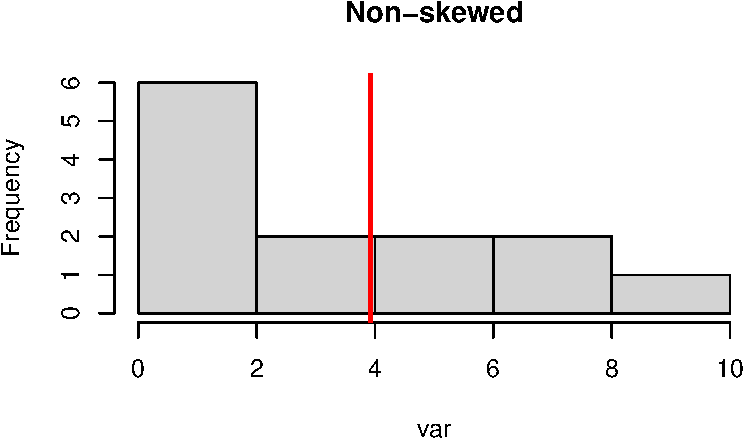
\includegraphics{stats_review_files/figure-pdf/unnamed-chunk-3-1.pdf}
\end{center}

\begin{Shaded}
\begin{Highlighting}[]
\FunctionTok{hist}\NormalTok{(var\_skewed, }\AttributeTok{breaks =} \DecValTok{30}\NormalTok{, }\AttributeTok{main =} \StringTok{"Skewed"}\NormalTok{)}
\FunctionTok{abline}\NormalTok{(}\AttributeTok{v =} \FunctionTok{mean}\NormalTok{(var\_skewed), }\AttributeTok{col=}\StringTok{"red"}\NormalTok{, }\AttributeTok{lwd=}\DecValTok{3}\NormalTok{)}
\end{Highlighting}
\end{Shaded}

\begin{center}
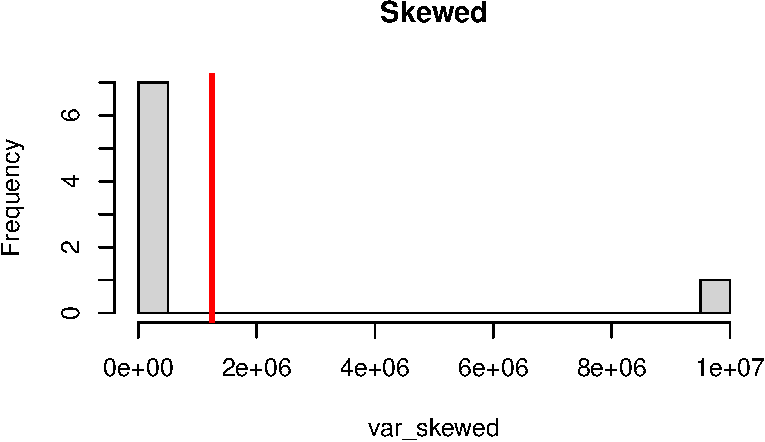
\includegraphics{stats_review_files/figure-pdf/unnamed-chunk-4-1.pdf}
\end{center}

Notice how in the figure above the mean does not do a good job at
identifying the value around which the data cluster. To improve on this,
we introduce the \emph{median}.

\subsubsection{Median}\label{median}

The
\href{https://www.khanacademy.org/math/statistics-probability/summarizing-quantitative-data/mean-median-basics/a/mean-median-and-mode-review\#:~:text=Median\%3A\%20The\%20middle\%20number\%3B\%20found,mean\%20of\%20those\%20two\%20numbers}{median}
is a measure of central tendency that is not sensitive to extreme values
in the dataset (a.k.a.,
\href{https://en.wikipedia.org/wiki/Outlier}{\emph{outliers}}). It
corresponds to the middle point in an ordered set of data (when the
total \(n\) is odd) or the mean of the two central middle observations
(when the total \(n\) is even). To show how this measure works, let's
take a look at how the median behaves when we plot it on the histogram
of our data.

\begin{Shaded}
\begin{Highlighting}[]
\FunctionTok{median}\NormalTok{(var)}
\end{Highlighting}
\end{Shaded}

\begin{verbatim}
[1] 3
\end{verbatim}

\begin{Shaded}
\begin{Highlighting}[]
\FunctionTok{median}\NormalTok{(var\_skewed)}
\end{Highlighting}
\end{Shaded}

\begin{verbatim}
[1] 1.5
\end{verbatim}

\begin{Shaded}
\begin{Highlighting}[]
\FunctionTok{hist}\NormalTok{(var, }\AttributeTok{main =} \StringTok{"Non{-}skewed"}\NormalTok{)}
\FunctionTok{abline}\NormalTok{(}\AttributeTok{v =} \FunctionTok{median}\NormalTok{(var), }\AttributeTok{col=}\StringTok{"red"}\NormalTok{, }\AttributeTok{lwd=}\DecValTok{3}\NormalTok{)}
\end{Highlighting}
\end{Shaded}

\begin{center}
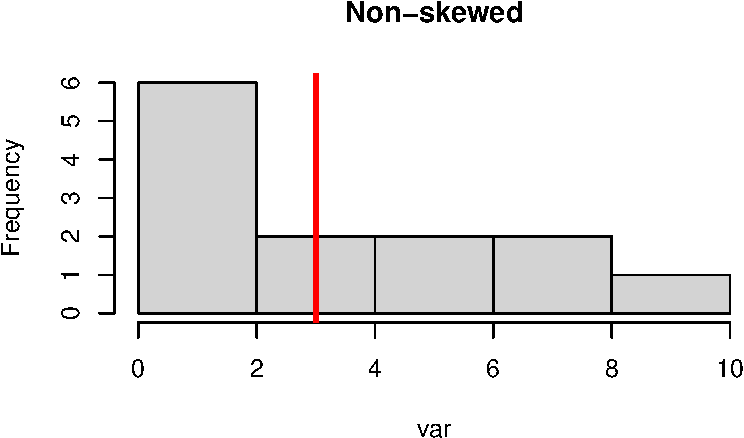
\includegraphics{stats_review_files/figure-pdf/unnamed-chunk-7-1.pdf}
\end{center}

\begin{Shaded}
\begin{Highlighting}[]
\FunctionTok{hist}\NormalTok{(var\_skewed, }\AttributeTok{breaks =} \DecValTok{30}\NormalTok{, }\AttributeTok{main =} \StringTok{"Skewed"}\NormalTok{)}
\FunctionTok{abline}\NormalTok{(}\AttributeTok{v =} \FunctionTok{median}\NormalTok{(var\_skewed), }\AttributeTok{col=}\StringTok{"red"}\NormalTok{, }\AttributeTok{lwd=}\DecValTok{3}\NormalTok{)}
\end{Highlighting}
\end{Shaded}

\begin{center}
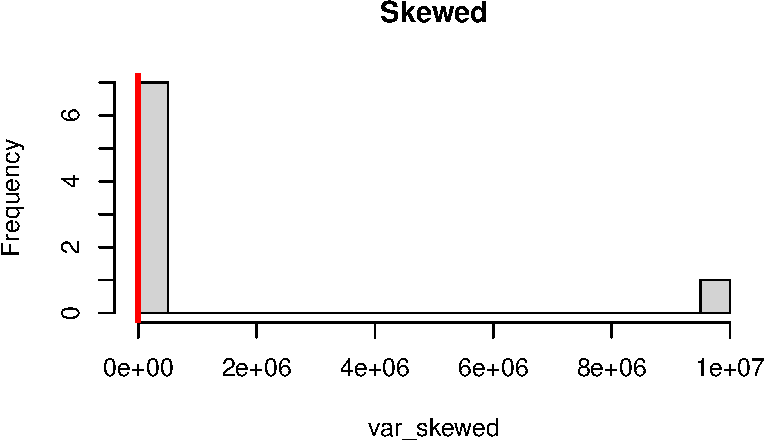
\includegraphics{stats_review_files/figure-pdf/unnamed-chunk-8-1.pdf}
\end{center}

from here you can clearly see that when data is highly skewed, the
median is able to better pinpoint where most of the data will be
located.

\subsubsection{Mode}\label{mode}

Finally, there is the mode which is simply the value of the observation
that occurs most frequently. Let's have a look at the sample data we
have to compute it. For that we can use the \texttt{table()} function in
R and pass in the variable \texttt{var} as an argument to it which will
return a
\href{https://www.ncl.ac.uk/webtemplate/ask-assets/external/maths-resources/statistics/data-presentation/frequency-distribution-tables.html\#:~:text=A\%20frequency\%20table\%20is\%20a,qualitative\%20or\%20quantitative\%20discrete\%20data.}{\emph{frequency
table}} showing how often each value appears in our variable.

\begin{Shaded}
\begin{Highlighting}[]
\FunctionTok{table}\NormalTok{(var)}
\end{Highlighting}
\end{Shaded}

\begin{verbatim}
var
1 2 3 4 5 6 7 8 9 
3 3 1 1 1 1 1 1 1 
\end{verbatim}

The mode for the variable above is not unique (both 1 and 2 are modes).
Indeed, the
\href{https://aarongullickson.github.io/stat_book/the-distribution-of-a-variable.html}{distribution}
of a variable might have one or more modes while others don't even have
one.

\begin{Shaded}
\begin{Highlighting}[]
\FunctionTok{table}\NormalTok{(var\_skewed)}
\end{Highlighting}
\end{Shaded}

\begin{verbatim}
var_skewed
    1     2     3     4 1e+07 
    4     1     1     1     1 
\end{verbatim}

Instead, for the case above, the mode is unique and is the value 1.

\begin{tcolorbox}[enhanced jigsaw, leftrule=.75mm, titlerule=0mm, toprule=.15mm, arc=.35mm, colframe=quarto-callout-note-color-frame, rightrule=.15mm, title=\textcolor{quarto-callout-note-color}{\faInfo}\hspace{0.5em}{Note}, opacitybacktitle=0.6, opacityback=0, bottomrule=.15mm, colback=white, toptitle=1mm, colbacktitle=quarto-callout-note-color!10!white, bottomtitle=1mm, left=2mm, breakable, coltitle=black]

As a side note, consider the following variable \(X\) which can take
values 1,2,3,4,5. Since each value appears with the same frequency
(e.g., \(\frac{1}{5}\)), \(X\) does not have a mode!

\end{tcolorbox}

\subsection{Measures of dispersion}\label{measures-of-dispersion}

It is also useful to quantify by how much variables vary on average.
These measures are often referred to as
\href{https://www.geeksforgeeks.org/measures-of-dispersion/}{measures of
dispersion} and there are a few which are fundamental for any
statistical application.

\subsubsection{Variance}\label{variance}

The \href{https://www.investopedia.com/terms/v/variance.asp}{variance}
of a variable measures the spread between its values and its mean.

\begin{equation}\phantomsection\label{eq-pop-variance}{
\sigma^2 = \frac{1}{N} \sum_{i=1}^N (x_i - \mu)^2
}\end{equation}

The term \((x_i - \mu)\) is often referred to as \emph{deviation from
the mean}. When we add all those up (notice the \(_i\) to the bottom
right of the \(x\)) and we square them we have a measure of how far
values of a variable are from their mean. Since we want an average
value, we divide the \emph{squared sum of all the deviations} by the
sample size \(N\).

\begin{tcolorbox}[enhanced jigsaw, leftrule=.75mm, titlerule=0mm, toprule=.15mm, arc=.35mm, colframe=quarto-callout-note-color-frame, rightrule=.15mm, title=\textcolor{quarto-callout-note-color}{\faInfo}\hspace{0.5em}{Note}, opacitybacktitle=0.6, opacityback=0, bottomrule=.15mm, colback=white, toptitle=1mm, colbacktitle=quarto-callout-note-color!10!white, bottomtitle=1mm, left=2mm, breakable, coltitle=black]

\(\mu\) is referred to as the
\href{https://www.wallstreetmojo.com/sample-mean-vs-population-mean/}{population
mean}.

Also, it is important to remember that the sum of all deviations from
the mean is 0. This is why we square them so as to avoid negative terms
in the sum and have a way to properly quantify the variance of a
variable.

\end{tcolorbox}

Variables with higher variance have values that are further away from
their mean on average. The opposite is true. In R we use the
\texttt{var()} function to compute the variance of a numeric variable
passed as argument in the function.

\phantomsection\label{annotated-cell-11}%
\begin{Shaded}
\begin{Highlighting}[]
\FunctionTok{var}\NormalTok{(var) }\hspace*{\fill}\NormalTok{\circled{1}}
\end{Highlighting}
\end{Shaded}

\begin{description}
\tightlist
\item[\circled{1}]
here the outside \texttt{var} refers to the variance function while the
\emph{var} inside the parenthesis is the argument to the function, which
in this case is our \emph{var}iable!
\end{description}

\begin{verbatim}
[1] 7.910256
\end{verbatim}

\begin{Shaded}
\begin{Highlighting}[]
\FunctionTok{var}\NormalTok{(var\_skewed) }\CommentTok{\#result is 12500000000000}
\end{Highlighting}
\end{Shaded}

\begin{verbatim}
[1] 1.25e+13
\end{verbatim}

Think about the two results above and make sure they make sense before
moving on! (Don't get confused by the
\href{https://calculator.name/scientific-notation-to-decimal/1.25e13}{scientific
notation} employed here by R in the output)

\begin{tcolorbox}[enhanced jigsaw, leftrule=.75mm, titlerule=0mm, toprule=.15mm, arc=.35mm, colframe=quarto-callout-caution-color-frame, rightrule=.15mm, title=\textcolor{quarto-callout-caution-color}{\faFire}\hspace{0.5em}{Caution}, opacitybacktitle=0.6, opacityback=0, bottomrule=.15mm, colback=white, toptitle=1mm, colbacktitle=quarto-callout-caution-color!10!white, bottomtitle=1mm, left=2mm, breakable, coltitle=black]

When computing the variance of a variable you have to keep in mind that
the resulting variance will be denominated by the square of the original
unit of measure.

For example, if my variable \(R\) representing the return on a stock is
denominated in \(USD\) its variance (\(Var[R]\)) will be denominated in
\(USD^2\). This makes the results less interpretable because in real
life there is no such thing as squared dollars!

Next we learn how to address this problem.

\end{tcolorbox}

\begin{tcolorbox}[enhanced jigsaw, leftrule=.75mm, titlerule=0mm, toprule=.15mm, arc=.35mm, colframe=quarto-callout-note-color-frame, rightrule=.15mm, title=\textcolor{quarto-callout-note-color}{\faInfo}\hspace{0.5em}{Note}, opacitybacktitle=0.6, opacityback=0, bottomrule=.15mm, colback=white, toptitle=1mm, colbacktitle=quarto-callout-note-color!10!white, bottomtitle=1mm, left=2mm, breakable, coltitle=black]

The formula for the variance introduced in
Equation~\ref{eq-pop-variance} is commonly referred to as the
\emph{population variance} of \(X\). Note that there is a difference
between this quantity and the sample variance which is computed as
follows:

\begin{equation}\phantomsection\label{eq-sample-var}{
s^2 = \frac{1}{n-1} \sum_{i=1}^n (x_i - \bar{x})^2
}\end{equation}

Notice the use of the \(s\) to represent a
\href{https://www.sciencedirect.com/topics/mathematics/sample-statistic}{sample
statistic}. Sample statistics are usually denoted by Latin alphabet
letters as opposed to population statistics denoted by letters from the
Greek alphabet.

Also, we are dividing by \(n-1\) due to the fact that we have one less
degree of freedom which has been used to compute the sample mean
\(\bar{x}\) as we use it to estimate the unknown population mean
\(\mu\).

\end{tcolorbox}

\subsubsection{Standard deviation}\label{standard-deviation}

Standard deviation is defined as the square root of the variance. This
solves the issue with the squared units of measures and brings
everything back to unit scale so that the results become easier to
interpret. In R you use \texttt{sd()} to compute the standard deviation
of a variable.

\begin{Shaded}
\begin{Highlighting}[]
\FunctionTok{sd}\NormalTok{(var)}
\end{Highlighting}
\end{Shaded}

\begin{verbatim}
[1] 2.812518
\end{verbatim}

\begin{Shaded}
\begin{Highlighting}[]
\FunctionTok{sd}\NormalTok{(var\_skewed)}
\end{Highlighting}
\end{Shaded}

\begin{verbatim}
[1] 3535533
\end{verbatim}

\subsubsection{Additional resources}\label{additional-resources}

We've seen most of the basics by now, but in case you want to learn more
about measures of dispersion here is a list of topics which you might
find useful:

\begin{enumerate}
\def\labelenumi{\arabic{enumi}.}
\tightlist
\item
  \href{https://www.scribbr.com/statistics/quartiles-quantiles/\#:~:text=A\%20quartile\%20is\%20a\%20type,sorted\%20data\%20into\%20q\%20parts.}{Quantiles
  and Quartiles}
\item
  \href{https://en.wikipedia.org/wiki/Interquartile_range}{Interquartile
  range}
\end{enumerate}

\subsubsection{The Two Variables Case}\label{the-two-variables-case}

Sometimes, we are not interested only in describing the behavior of a
single variable but we might want to study how it interacts with another
variable. Quantifying this relationship is very easy thanks to some
tools such as the \textbf{covariance} of two variables and the
\textbf{correlation coefficient}.

\paragraph{Covariance}\label{covariance}

Covariance refers to how much two variables co-vary (i.e., vary
together). It is useful to look at the formula of how it is computed to
derive some intuition about how it works.

\[
\text{Cov}(X, Y) = \frac{1}{n} \sum_{i=1}^{n} (x_i - \bar{x})(y_i - \bar{y})
\]

In other words, the covariance of two variables \(X\) and \(Y\) is
determined by how many times they are both above (or below) their
respective means, \(\bar{x}\) and \(\bar{y}\). Intuitively, if they are
both above (or below) their mean we would be multiplying together two
numbers with the same sign, and the result will be a positive number.
Then, following simple reasoning, if we add together many positive
numbers we get a number that is larger than if we were to add an equal
number of some negative and some positive numbers together (assuming
they are the same in absolute value). It follows that two variables that
are more often than not above their means, at the same time, will have a
higher covariance, meaning that these variables will be growing (or
shrinking) together.

The opposite of this is the case when two variables have a covariance
that is close to 0, which is the same as saying that the two variables
are independent (i.e., knowing that one of the variables changes tells
me nothing about how the other behaves).

\begin{tcolorbox}[enhanced jigsaw, leftrule=.75mm, titlerule=0mm, toprule=.15mm, arc=.35mm, colframe=quarto-callout-caution-color-frame, rightrule=.15mm, title=\textcolor{quarto-callout-caution-color}{\faFire}\hspace{0.5em}{Caution}, opacitybacktitle=0.6, opacityback=0, bottomrule=.15mm, colback=white, toptitle=1mm, colbacktitle=quarto-callout-caution-color!10!white, bottomtitle=1mm, left=2mm, breakable, coltitle=black]

Covariance has the same issue that variance has: squared units of
measure. We learn how to deal with this next.

\end{tcolorbox}

\paragraph{Correlation coefficient}\label{correlation-coefficient}

In a similar way to how the standard deviation solves the issue of
squared units of measures for the variance, so does the correlation
coefficient for the covariance. Here is its formula:

\[
r = \frac{\operatorname{Cov}(X, Y)}{\sigma_X \sigma_Y}
\]

From here, we notice some important properties of \(r\):

\begin{enumerate}
\def\labelenumi{\arabic{enumi}.}
\tightlist
\item
  It is scaled (i.e., divided) by the product of the standard deviation
  of the two variables, and therefore \(r\) now always falls in the
  range {[}-1,1{]}. This allows us to have boundaries to interpret the
  strength of the relationship between \(X\) and \(Y\).
\item
  The closer \(|r|\) is to 1 (in
  \href{https://en.wikipedia.org/wiki/Absolute_value}{absolute value})
  the stronger the relationship between the two variables.
\item
  The sign of \(r\) is determined solely by the sign of the
  \(\operatorname{Cov}(X, Y)\) at the numerator since the standard
  deviations at the bottom are always positive values.
\end{enumerate}

\begin{tcolorbox}[enhanced jigsaw, leftrule=.75mm, titlerule=0mm, toprule=.15mm, arc=.35mm, colframe=quarto-callout-important-color-frame, rightrule=.15mm, title=\textcolor{quarto-callout-important-color}{\faExclamation}\hspace{0.5em}{Important}, opacitybacktitle=0.6, opacityback=0, bottomrule=.15mm, colback=white, toptitle=1mm, colbacktitle=quarto-callout-important-color!10!white, bottomtitle=1mm, left=2mm, breakable, coltitle=black]

Notice that \(r\) measures the strength of \emph{linear correlation}
between two variables. This means that if \(X\) and \(Y\) are linked by
a non-linear relationship, \(r\) will not be able to detect it! We show
this with an example.

\end{tcolorbox}

\phantomsection\label{annotated-cell-15}%
\begin{Shaded}
\begin{Highlighting}[]
\NormalTok{lin\_1 }\OtherTok{\textless{}{-}} \FunctionTok{seq}\NormalTok{(}\DecValTok{1}\NormalTok{,}\DecValTok{10}\NormalTok{) }\hspace*{\fill}\NormalTok{\circled{1}}
\NormalTok{lin\_2 }\OtherTok{\textless{}{-}} \FunctionTok{seq}\NormalTok{(}\SpecialCharTok{{-}}\DecValTok{1}\NormalTok{,}\SpecialCharTok{{-}}\DecValTok{10}\NormalTok{) }\hspace*{\fill}\NormalTok{\circled{2}}

\FunctionTok{cor}\NormalTok{(lin\_1, lin\_2) }\hspace*{\fill}\NormalTok{\circled{3}}
\end{Highlighting}
\end{Shaded}

\begin{description}
\tightlist
\item[\circled{1}]
generate sequence of numbers from 1 to 10
\item[\circled{2}]
generate sequence of numbers from -1 to -10
\item[\circled{3}]
compute the \texttt{cor}relation between these two linear sequences
\end{description}

\begin{verbatim}
[1] -1
\end{verbatim}

\phantomsection\label{annotated-cell-16}%
\begin{Shaded}
\begin{Highlighting}[]
\NormalTok{sq\_2 }\OtherTok{\textless{}{-}}\NormalTok{ lin\_1}\SpecialCharTok{\^{}}\DecValTok{2} \hspace*{\fill}\NormalTok{\circled{1}}

\FunctionTok{cor}\NormalTok{(lin\_1, sq\_2) }\hspace*{\fill}\NormalTok{\circled{2}}
\end{Highlighting}
\end{Shaded}

\begin{description}
\tightlist
\item[\circled{1}]
\texttt{sq\_2} is the square of the sequence of numbers from 1 to 10
contained in \texttt{lin\_1}.
\item[\circled{2}]
the correlation coefficient computed will now have more troubles
recognizing this
\href{https://en.wikipedia.org/wiki/Quadratic_equation}{non-linear
relationship} and produce a lower correlation coefficient (in absolute
value).
\end{description}

\begin{verbatim}
[1] 0.9745586
\end{verbatim}

\section{Inferential statistics}\label{inferential-statistics}

Inferential statistics refers to how we can make
\href{https://www.merriam-webster.com/dictionary/inference}{inferences}
about a population starting from a
\href{https://www.investopedia.com/terms/r/representative-sample.asp\#:~:text=A\%20representative\%20sample\%20is\%20a,three\%20males\%20and\%20three\%20females.}{representative
sample} drawn from it.

\subsection{Probability Distributions}\label{probability-distributions}

\href{https://en.wikipedia.org/wiki/Probability_theory}{Probability
theory} refers to the set of tools mathematicians developed to study and
model uncertainty. Here we are just going to introduce elementary topics
to not make things too complicated.

When we try to understand what are the chances that something happen or
does not happen, we are basically questioning whether an \emph{event}
will or will not take place. An event is an observable outcome which can
either happen or not. For instance, if my event \(A\) is defined as
observing a 2 on a single die roll it can either happen (I roll the die
and I get a 2) or it does not happen (I get a number other than 2). Now,
assuming that the die is fair (i.e., every number as an equal chance to
show), we can assign a probability to the event that we get a 2, denoted
by \(P(A) = \frac{1}{6}\) (meaning there is just \textbf{a single 2},
over a \textbf{total of 6 possible numbers} that I can get from a single
die roll). In general, we can denote by \(X\) a random variable that
takes on each roll the value of the observed number. Then, \(X\) is
random because its value cannot be predetermined exactly
\href{https://en.wikipedia.org/wiki/A_priori_and_a_posteriori}{\emph{a
priori}} but is the result of the following die roll.

\subsubsection{Binomial distribution}\label{binomial-distribution}

Knowing this, we can use a probability distribution to compute the
probability that we observe a specific number of 2's over a series of
\(n\) die rolls. This is an example of a
\href{https://www.statisticshowto.com/probability-and-statistics/binomial-theorem/binomial-experiment/}{binomial
experiment}. If you are interested you can learn more about it but for
now it suffices to say that we can model this using a
\href{https://en.wikipedia.org/wiki/Binomial_distribution}{binomial
distribution}. Plotting the distribution we observe that rolling the die
100 times yields the following.

\begin{Shaded}
\begin{Highlighting}[]
\FunctionTok{set.seed}\NormalTok{(}\DecValTok{126}\NormalTok{)}
\NormalTok{possible\_outcomes }\OtherTok{\textless{}{-}} \FunctionTok{seq}\NormalTok{(}\DecValTok{1}\NormalTok{,}\DecValTok{6}\NormalTok{)}
\NormalTok{observed\_outcomes }\OtherTok{\textless{}{-}} \FunctionTok{sample}\NormalTok{(possible\_outcomes, }\AttributeTok{size =} \DecValTok{100}\NormalTok{, }
                            \AttributeTok{replace =}\NormalTok{ T, }\AttributeTok{prob =} \FunctionTok{c}\NormalTok{(}\DecValTok{1}\SpecialCharTok{/}\DecValTok{6}\NormalTok{,}\DecValTok{1}\SpecialCharTok{/}\DecValTok{6}\NormalTok{,}\DecValTok{1}\SpecialCharTok{/}\DecValTok{6}\NormalTok{,}\DecValTok{1}\SpecialCharTok{/}\DecValTok{6}\NormalTok{,}\DecValTok{1}\SpecialCharTok{/}\DecValTok{6}\NormalTok{,}\DecValTok{1}\SpecialCharTok{/}\DecValTok{6}\NormalTok{))}

\FunctionTok{hist}\NormalTok{(observed\_outcomes, }\AttributeTok{breaks =} \FunctionTok{c}\NormalTok{(}\DecValTok{0}\NormalTok{,}\DecValTok{1}\NormalTok{,}\DecValTok{2}\NormalTok{,}\DecValTok{3}\NormalTok{,}\DecValTok{4}\NormalTok{,}\DecValTok{5}\NormalTok{,}\DecValTok{6}\NormalTok{), }\AttributeTok{freq =}\NormalTok{ F, }
     \AttributeTok{labels =}\NormalTok{ T, }\AttributeTok{ylim =} \FunctionTok{c}\NormalTok{(}\DecValTok{0}\NormalTok{,.}\DecValTok{3}\NormalTok{))}
\end{Highlighting}
\end{Shaded}

\begin{center}
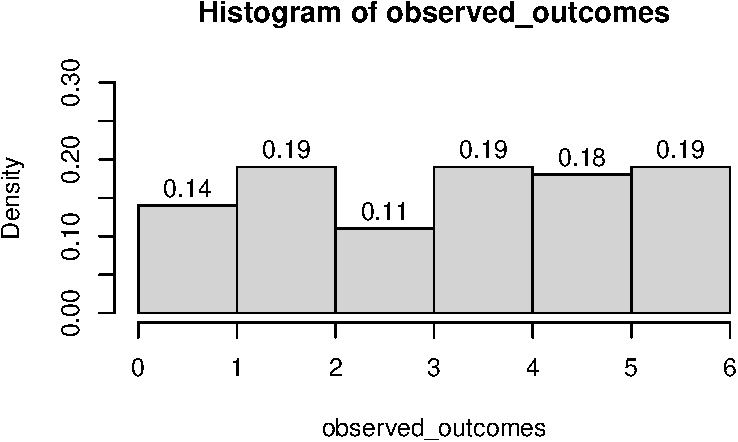
\includegraphics{stats_review_files/figure-pdf/unnamed-chunk-17-1.pdf}
\end{center}

In this case 19\% of all rolls (meaning 19 rolls) produced had as an
outcome a 2. We could have computed this probability before conducting
the experiment so as to form an expectation of what the outcome of the
die roll would more likely be by multiplying the probability of
observing a 2 on a die roll (\(p=\frac{1}{6}\)) by the number of times
the die is rolled (\(n=100\)) and the expected numbers of 2 would have
been approximately 17, not that far from what we observed!

\subsubsection{Normal distribution}\label{normal-distribution}

If you had to learn about only one distribution, let that be the
\href{https://www.investopedia.com/terms/n/normaldistribution.asp\#:~:text=The\%20Bottom\%20Line-,Normal\%20distribution\%2C\%20also\%20known\%20as\%20the\%20Gaussian\%20distribution\%2C\%20is\%20a,defined\%20by\%20the\%20standard\%20deviation.}{Normal
Distribution}. There are so many important things there are to say about
this distribution, but let's keep it simple:

\begin{enumerate}
\def\labelenumi{\arabic{enumi}.}
\tightlist
\item
  it is used to model many real-life phenomena that take on a
  \href{https://www.google.com/url?sa=t&source=web&rct=j&opi=89978449&url=https://www.youtube.com/watch\%3Fv\%3DQxqxdQ_g2uw&ved=2ahUKEwithPq87daJAxVr_7sIHWqJG7QQwqsBegQIMRAF&usg=AOvVaw0dJpzZRYGkC9qx1omRy_Xa}{continuum
  of values} (and not a discrete number of values, like the previous die
  roll example)
\item
  it depends on only two parameters: its mean (\$\mu\$), and its
  variance (\$\sigma\^{}2\$)
\item
  given some assumptions, any distribution can be approximated by the
  Normal Distribution! This is a result of the
  \href{https://www.investopedia.com/terms/c/central_limit_theorem.asp}{Central
  Limit Theorem}.
\item
  it has many nice properties (symmetry about \(\mu\), bell shape, etc.)
  and is used all over statistics and forecasting, along with its sample
  counterpart being the
  \href{https://www.investopedia.com/terms/t/tdistribution.asp}{T
  distribution}
\end{enumerate}

Let's plot it out

\begin{Shaded}
\begin{Highlighting}[]
\NormalTok{x }\OtherTok{\textless{}{-}} \FunctionTok{seq}\NormalTok{(}\SpecialCharTok{{-}}\DecValTok{4}\NormalTok{,}\DecValTok{4}\NormalTok{,.}\DecValTok{001}\NormalTok{)}
\NormalTok{y }\OtherTok{\textless{}{-}} \FunctionTok{dnorm}\NormalTok{(x)}

\FunctionTok{plot}\NormalTok{(x,y, }\AttributeTok{main =} \StringTok{"The Standard Normal Distribution"}\NormalTok{)}
\FunctionTok{abline}\NormalTok{(}\AttributeTok{v=}\FunctionTok{mean}\NormalTok{(x), }\AttributeTok{col =} \StringTok{"red"}\NormalTok{, }\AttributeTok{lwd=}\DecValTok{2}\NormalTok{)}
\end{Highlighting}
\end{Shaded}

\begin{center}
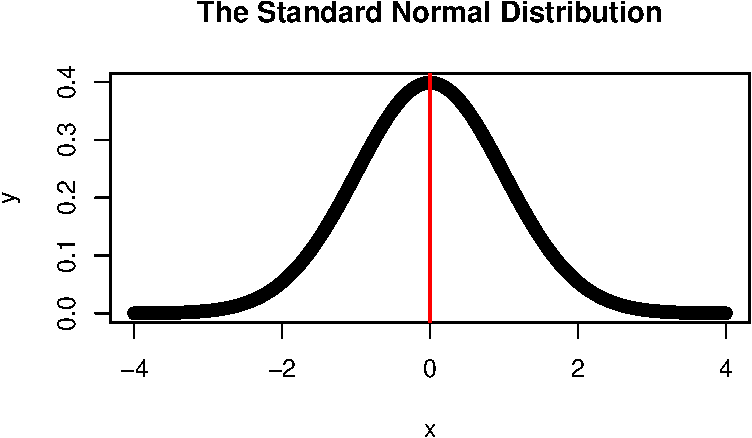
\includegraphics{stats_review_files/figure-pdf/unnamed-chunk-18-1.pdf}
\end{center}

there is also a special case of the normal distribution which occurs
when \(\mu=0\) and \(\sigma^2=1\). This is called the
\href{https://www.scribbr.com/statistics/standard-normal-distribution/}{standard
normal distribution} (represented by \(Z\)). This means that one can
\href{https://www.listendata.com/2017/04/how-to-standardize-variable-in-regression.html}{\emph{standardize}}
any normal random variable to bring it back to this standard scale and
obtain a distribution like the one above. To do that, you simply need to
subtract the \emph{mean} of the variable you are standardizing and
divide by its \emph{standard deviation}.

\[
Z = \frac{X - \mu}{\sigma}
\]

\subsubsection{Student's T distribution}\label{students-t-distribution}

Another useful distribution is the
\href{https://en.wikipedia.org/wiki/Student\%27s_t-distribution}{T
distribution}. Shape-wise the T distribution has the same nice
properties of the standard normal distribution (of which it is a
generalization). However, it is common to use this distribution when we
do not know the true population value of \(\sigma^2\) and we have to use
its sample counterpart \(s^{2}\) as its estimate. The T distribution
comes with
\href{https://www.scribbr.com/statistics/degrees-of-freedom/\#:~:text=Degrees\%20of\%20freedom\%2C\%20often\%20represented,minus\%20the\%20number\%20of\%20restrictions.}{degrees
of freedom} which are used to assess how many data points are left free
to vary after having estimated the population parameters that we need
from the sample. In this case, note that since we are using \(\bar{x}\)
to estimate \(\mu\) we lose one degree of freedom and our T distribution
will be defined by \(n-1\) degrees of freedom. To be convinced of this
you can take another look at Equation~\ref{eq-sample-var} and notice
that the \(\mu\) is replaced by \(\bar{x}\).

\subsection{Hypothesis Testing}\label{sec-testhyp}

\subsubsection{One-sided tests}\label{sec-one-sided-tests}

Given two groups of people, you might be interested in understanding
which group is taller on average. This can be translated into a test of
hypothesis. Let's say you believe group 1 to be taller on average, how
would you go about testing this quantitatively? First, let's define the
two hypotheses:

\[
H_0: \mu_1 \leq \mu_2
\]

\[
H_1: \mu_1 > \mu_2
\]

Let's break this down:

\begin{enumerate}
\def\labelenumi{\arabic{enumi}.}
\tightlist
\item
  Here \(H_0\) is known as the
  \href{https://en.wikipedia.org/wiki/Null_hypothesis}{null hypothesis},
  and it represents the
  \href{https://www.vocabulary.com/dictionary/status\%20quo}{status quo}
  or what we assume to be the truth.
\item
  \(H_1\) is the
  \href{https://en.wikipedia.org/wiki/Alternative_hypothesis}{alternative}
  (or research) hypothesis, and it is what we want to find evidence for.
  Note that finding supporting evidence for \(H_1\) makes \(H_0\) less
  credible. This derives from the way in which the two hypotheses are
  constructed and how one must necessarily be the complement of the
  other in order for this method to work.
\item
  \(\mu_i\) for \(i = {1,2}\) represents the theoretical population mean
  of group 1 and 2, which we are trying to infer from our sample data.
\end{enumerate}

Also, notice that the system of hypothesis reported below is the same as
the one proposed above and you can easily check this using basic
algebra.

\[
H_0: \mu_1 -\mu_2 \le 0
\]

\[
H_1: \mu_1 -\mu_2 > 0
\]

This formulation is more useful as it reduces everything to a difference
between the means of the two groups.

\begin{tcolorbox}[enhanced jigsaw, leftrule=.75mm, titlerule=0mm, toprule=.15mm, arc=.35mm, colframe=quarto-callout-important-color-frame, rightrule=.15mm, title=\textcolor{quarto-callout-important-color}{\faExclamation}\hspace{0.5em}{Important}, opacitybacktitle=0.6, opacityback=0, bottomrule=.15mm, colback=white, toptitle=1mm, colbacktitle=quarto-callout-important-color!10!white, bottomtitle=1mm, left=2mm, breakable, coltitle=black]

This system of hypothesis is referred to as a \emph{one-sided test of
hypothesis}. This means that we are only interested in finding
contradiction to \(H_0\) in one direction (in this case in the upper
tail). The direction in which we seek contradiction to \(H_0\) is
determined by the inequality sign used in \(H_1\).

\end{tcolorbox}

Now, it would be useful to have a metric that could help us determine
whether there is enough supporting evidence for \(H_1\) to \emph{reject}
\(H_0\). To do this, we introduce the concepts of
\href{https://en.wikipedia.org/wiki/Statistical_significance}{significance
level} (denoted by \(\alpha\)) and
\href{https://www.scribbr.com/statistics/p-value/\#:~:text=A\%20p\%2Dvalue\%2C\%20or\%20probability,to\%20perform\%20your\%20statistical\%20test.}{p-value}
(denoted by \(p\)). The p-value of a test is the probability of
observing the result that we actually observed (from sample data) if we
assume the null hypothesis to be true. Of course, a small p-value tells
us that what we observed is unlikely to happen if the null hypothesis
was effectively true. How small the p-value needs to be to reject
\(H_0\) depends on the significance level we are using for our tests.
Commonly, the .01, .05, and .1 significance levels are the most used
ones, but there are scientific fields that require even smaller
\(\alpha\) (e.g.,
\href{https://home.cern/resources/faqs/five-sigma}{physics}). Given the
concepts of p-value and significance level just discussed, the following
method is used to determine whether one should reject or do not reject
the null hypothesis:

\begin{tcolorbox}[enhanced jigsaw, leftrule=.75mm, titlerule=0mm, toprule=.15mm, arc=.35mm, colframe=quarto-callout-important-color-frame, rightrule=.15mm, title=\textcolor{quarto-callout-important-color}{\faExclamation}\hspace{0.5em}{Important}, opacitybacktitle=0.6, opacityback=0, bottomrule=.15mm, colback=white, toptitle=1mm, colbacktitle=quarto-callout-important-color!10!white, bottomtitle=1mm, left=2mm, breakable, coltitle=black]

\begin{enumerate}
\def\labelenumi{\arabic{enumi}.}
\tightlist
\item
  If \(p < \alpha \rightarrow\) reject \(H_0\)
\item
  if \(p > \alpha \rightarrow\) do not reject \(H_0\)
\end{enumerate}

\end{tcolorbox}

To go back to our original height problem and to determine whether group
1 is truly taller on average compared to group 2 we need to introduce
the t-statistic. The t-statistic comes from the \(T\) distribution and
it is used to quantify by how much two sample means differ from each
other.

\phantomsection\label{annotated-cell-19}%
\begin{Shaded}
\begin{Highlighting}[]
\FunctionTok{set.seed}\NormalTok{(}\DecValTok{128}\NormalTok{) }\hspace*{\fill}\NormalTok{\circled{1}}
\NormalTok{pop\_1 }\OtherTok{\textless{}{-}} \FunctionTok{seq}\NormalTok{(}\DecValTok{180}\NormalTok{,}\DecValTok{195}\NormalTok{) }\hspace*{\fill}\NormalTok{\circled{2}}
\NormalTok{pop\_2 }\OtherTok{\textless{}{-}} \FunctionTok{seq}\NormalTok{(}\DecValTok{165}\NormalTok{,}\DecValTok{180}\NormalTok{) }\hspace*{\fill}\NormalTok{\circled{3}}

\NormalTok{sample\_1 }\OtherTok{\textless{}{-}} \FunctionTok{sample}\NormalTok{(pop\_1, }\DecValTok{100}\NormalTok{, }\AttributeTok{replace =}\NormalTok{ T) }\hspace*{\fill}\NormalTok{\circled{4}}
\NormalTok{sample\_2 }\OtherTok{\textless{}{-}} \FunctionTok{sample}\NormalTok{(pop\_2, }\DecValTok{100}\NormalTok{, }\AttributeTok{replace =}\NormalTok{ T) }\hspace*{\fill}\NormalTok{\circled{5}}
\end{Highlighting}
\end{Shaded}

\begin{description}
\tightlist
\item[\circled{1}]
Set the seed to get reproducible results across iterations
\item[\circled{2}]
specify that population 1 is made up of individuals with height between
180cm and 195cm
\item[\circled{3}]
specify that population 2 is made up of individuals with height between
165cm and 180cm
\item[\circled{4}]
sample 100 elements \emph{with replacement} (i.e., allowing for the same
value to be drawn multiple times) from population 1
\item[\circled{5}]
sample 100 elements \emph{with replacement} from population 2
\end{description}

Let's plot the distribution of the height of the two samples.

\begin{Shaded}
\begin{Highlighting}[]
\FunctionTok{hist}\NormalTok{(sample\_1)}
\FunctionTok{abline}\NormalTok{(}\AttributeTok{v=}\FunctionTok{mean}\NormalTok{(sample\_1), }\AttributeTok{col=}\StringTok{"red"}\NormalTok{, }\AttributeTok{lwd=}\DecValTok{3}\NormalTok{)}
\end{Highlighting}
\end{Shaded}

\begin{center}
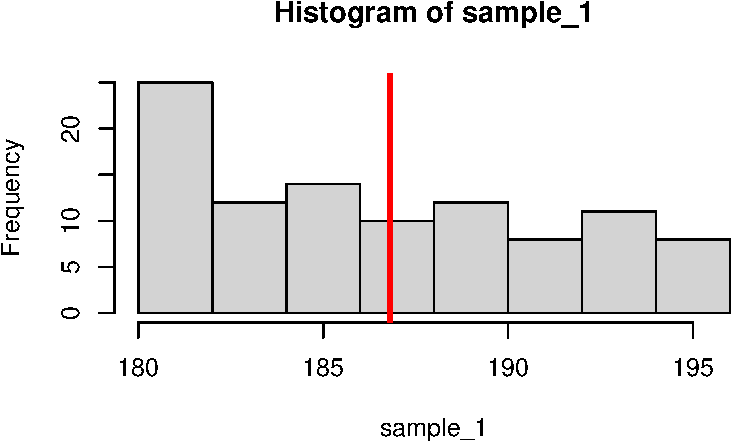
\includegraphics{stats_review_files/figure-pdf/unnamed-chunk-20-1.pdf}
\end{center}

\begin{Shaded}
\begin{Highlighting}[]
\FunctionTok{hist}\NormalTok{(sample\_2, }\AttributeTok{xlim =} \FunctionTok{c}\NormalTok{(}\DecValTok{164}\NormalTok{,}\DecValTok{180}\NormalTok{))}
\FunctionTok{abline}\NormalTok{(}\AttributeTok{v=}\FunctionTok{mean}\NormalTok{(sample\_2), }\AttributeTok{col=}\StringTok{"red"}\NormalTok{, }\AttributeTok{lwd=}\DecValTok{3}\NormalTok{)}
\end{Highlighting}
\end{Shaded}

\begin{center}
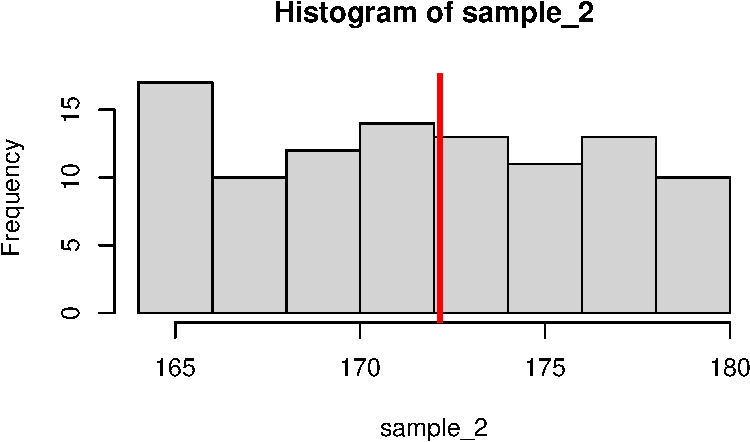
\includegraphics{stats_review_files/figure-pdf/unnamed-chunk-21-1.pdf}
\end{center}

Finally, we conduct a t-test to determine whether there is a significant
difference in means between the two samples.

\begin{Shaded}
\begin{Highlighting}[]
\NormalTok{(t\_test }\OtherTok{\textless{}{-}} \FunctionTok{t.test}\NormalTok{(sample\_1, sample\_2, }\AttributeTok{alternative =} \StringTok{"greater"}\NormalTok{))}
\end{Highlighting}
\end{Shaded}

\begin{verbatim}

    Welch Two Sample t-test

data:  sample_1 and sample_2
t = 21.546, df = 197.8, p-value < 2.2e-16
alternative hypothesis: true difference in means is greater than 0
95 percent confidence interval:
 13.52635      Inf
sample estimates:
mean of x mean of y 
   186.81    172.16 
\end{verbatim}

\begin{Shaded}
\begin{Highlighting}[]
\NormalTok{t\_test}\SpecialCharTok{$}\NormalTok{p.value}
\end{Highlighting}
\end{Shaded}

\begin{verbatim}
[1] 4.361519e-54
\end{verbatim}

Given a level of significance \(\alpha\) = .01 and a \(p\) \textless{}
.001 we can reject \(H_0\). This means that under the assumption that
\(H_0\) is true, we would be less than 0.1\% likely to observe the
height distributions that we ended up observing in the two groups. For
this reason, \(H_0\) does not seem to reflect well what we observed in
our experiment and therefore is rejected.

\begin{tcolorbox}[enhanced jigsaw, leftrule=.75mm, titlerule=0mm, toprule=.15mm, arc=.35mm, colframe=quarto-callout-important-color-frame, rightrule=.15mm, title=\textcolor{quarto-callout-important-color}{\faExclamation}\hspace{0.5em}{Important}, opacitybacktitle=0.6, opacityback=0, bottomrule=.15mm, colback=white, toptitle=1mm, colbacktitle=quarto-callout-important-color!10!white, bottomtitle=1mm, left=2mm, breakable, coltitle=black]

Tests of hypotheses are everywhere in inferential statistics, so be sure
to have familiarized with what discussed in this section.

\end{tcolorbox}

\subsubsection{Two-sided tests}\label{sec-two-sided-tests}

Suppose now instead that we are interested in testing the following
system of hypotheses:

\[
H_0: \mu_1 = \mu_2
\]

\[
H_1: \mu_1 \neq \mu_2
\]

In this case finding contradiction to \(H_0\) is the same as finding a
large difference in the two means (in absolute value). Therefore, it
does not matter whether it is a positive or a negative difference! When
this happens, we say that we conduct a \emph{two-sided test of
hypothesis}.

Using the same data as before, we can test this new hypothesis in the
following way:

\begin{Shaded}
\begin{Highlighting}[]
\NormalTok{(t\_test }\OtherTok{\textless{}{-}} \FunctionTok{t.test}\NormalTok{(sample\_1, sample\_2))}
\end{Highlighting}
\end{Shaded}

\begin{verbatim}

    Welch Two Sample t-test

data:  sample_1 and sample_2
t = 21.546, df = 197.8, p-value < 2.2e-16
alternative hypothesis: true difference in means is not equal to 0
95 percent confidence interval:
 13.30916 15.99084
sample estimates:
mean of x mean of y 
   186.81    172.16 
\end{verbatim}

And we get the following p-value:

\begin{Shaded}
\begin{Highlighting}[]
\NormalTok{t\_test}\SpecialCharTok{$}\NormalTok{p.value}
\end{Highlighting}
\end{Shaded}

\begin{verbatim}
[1] 8.723038e-54
\end{verbatim}

\subsubsection{A note about p-values}\label{a-note-about-p-values}

Following the interpretation given in Section~\ref{sec-one-sided-tests},
a generic p-value for a test can be computed after obtaining a feasible
test statistic from the data for which we know the distribution. In the
case of the hypothesis tests about two population means discussed above,
that test statistic is given by the t-value for which we know the
reference distribution (i.e., Student's \(T\)). Then, given a
distribution and its parameters, we can compute the p-value as the
probability of observing values more extreme as the one observed.
Namely, in the case of the test discussed in
Section~\ref{sec-one-sided-tests} we want to find \(P(T_{df} > t)\)
where \(t\) stands for the computed t-value of the test. An example of
computing the p-value manually follows below:

\begin{Shaded}
\begin{Highlighting}[]
\FunctionTok{pt}\NormalTok{(}\FloatTok{21.546}\NormalTok{, }\FloatTok{197.8}\NormalTok{, }\AttributeTok{lower.tail =}\NormalTok{ F)}
\end{Highlighting}
\end{Shaded}

\begin{verbatim}
[1] 4.368875e-54
\end{verbatim}

Instead, a p-value for the test proposed in
Section~\ref{sec-two-sided-tests} can be found by multiplying the
probability found above by 2: \(2P(T_{df} > t)\), so that the
computation reduces to:

\begin{Shaded}
\begin{Highlighting}[]
\DecValTok{2}\SpecialCharTok{*}\FunctionTok{pt}\NormalTok{(}\FloatTok{21.546}\NormalTok{, }\FloatTok{197.8}\NormalTok{, }\AttributeTok{lower.tail =}\NormalTok{ F)}
\end{Highlighting}
\end{Shaded}

\begin{verbatim}
[1] 8.73775e-54
\end{verbatim}

The reason why this applies is due to the symmetry of the \(T\)
distribution. You can see from the figure below that the area under the
curve below the value -2 and above 2 is the same.

\begin{Shaded}
\begin{Highlighting}[]
\NormalTok{x }\OtherTok{\textless{}{-}} \FunctionTok{seq}\NormalTok{(}\SpecialCharTok{{-}}\DecValTok{3}\NormalTok{,}\DecValTok{3}\NormalTok{,.}\DecValTok{01}\NormalTok{)}
\NormalTok{y }\OtherTok{\textless{}{-}} \FunctionTok{dt}\NormalTok{(x, }\DecValTok{100}\NormalTok{)}

\FunctionTok{plot}\NormalTok{(x,y, }\AttributeTok{main =} \StringTok{"Density of T Distribution w/ 100 df"}\NormalTok{, }\AttributeTok{ylab =} \StringTok{"density"}\NormalTok{)}
\FunctionTok{abline}\NormalTok{(}\AttributeTok{v =} \DecValTok{2}\NormalTok{, }\AttributeTok{col =} \StringTok{"red"}\NormalTok{, }\AttributeTok{lwd =} \DecValTok{2}\NormalTok{)}
\FunctionTok{abline}\NormalTok{(}\AttributeTok{v =} \SpecialCharTok{{-}}\DecValTok{2}\NormalTok{, }\AttributeTok{col =} \StringTok{"red"}\NormalTok{, }\AttributeTok{lwd =} \DecValTok{2}\NormalTok{)}
\end{Highlighting}
\end{Shaded}

\begin{center}
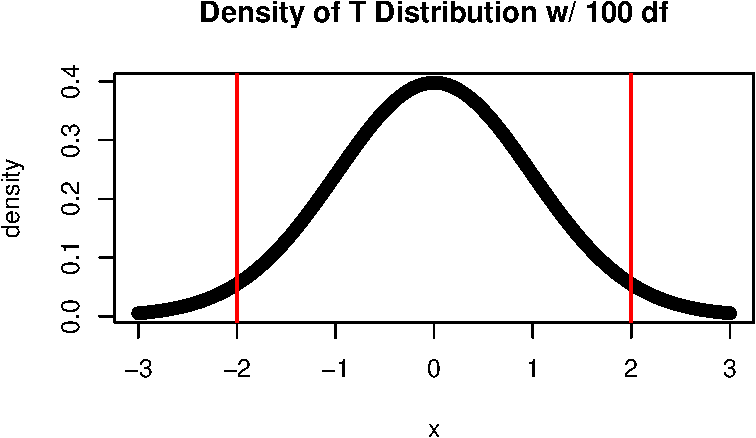
\includegraphics{stats_review_files/figure-pdf/unnamed-chunk-28-1.pdf}
\end{center}

You can check that the p-values computed following this approach are
practically equal to the ones found with the \texttt{t.test} function in
Section~\ref{sec-one-sided-tests} and Section~\ref{sec-two-sided-tests}

\subsection{(Linear) Regression}\label{linear-regression}

A linear regression is a model which estimates the (linear) relationship
between one variable (dependent variable) and at least one other
variable (independent variable). Linear regression is useful in that it
quantifies how much the dependent variable changes as we let the
independent variable(s) change. We now have a look at what should be
clear about all this.

\subsubsection{Simple regression}\label{simple-regression}

A simple regression is a regression model with a single independent
variable. The equation that describes these models is usually of the
form:

\[
\hat Y_i = \hat\beta_0 + \hat\beta_1X_i
\]

Where \(\hat Y_i\) is the predicted value of \(Y\) when the independent
variable \(X\) takes value \(X_i\) and it is multiplied by the estimated
slope parameter \(\hat\beta_1\) and added to the estimated intercept
parameter \(\hat\beta_0\). We now have a look at it in code.

\phantomsection\label{annotated-cell-29}%
\begin{Shaded}
\begin{Highlighting}[]
\FunctionTok{library}\NormalTok{(MASS) }\hspace*{\fill}\NormalTok{\circled{1}}
\NormalTok{(animals }\OtherTok{\textless{}{-}}\NormalTok{ MASS}\SpecialCharTok{::}\NormalTok{Animals) }\hspace*{\fill}\NormalTok{\circled{2}}
\end{Highlighting}
\end{Shaded}

\begin{description}
\tightlist
\item[\circled{1}]
import the library \texttt{MASS}
\item[\circled{2}]
get the Animals dataset from inside the \texttt{MASS} library and assign
it to the variable \texttt{animals}
\end{description}

\begin{verbatim}
                      body  brain
Mountain beaver      1.350    8.1
Cow                465.000  423.0
Grey wolf           36.330  119.5
Goat                27.660  115.0
Guinea pig           1.040    5.5
Dipliodocus      11700.000   50.0
Asian elephant    2547.000 4603.0
Donkey             187.100  419.0
Horse              521.000  655.0
Potar monkey        10.000  115.0
Cat                  3.300   25.6
Giraffe            529.000  680.0
Gorilla            207.000  406.0
Human               62.000 1320.0
African elephant  6654.000 5712.0
Triceratops       9400.000   70.0
Rhesus monkey        6.800  179.0
Kangaroo            35.000   56.0
Golden hamster       0.120    1.0
Mouse                0.023    0.4
Rabbit               2.500   12.1
Sheep               55.500  175.0
Jaguar             100.000  157.0
Chimpanzee          52.160  440.0
Rat                  0.280    1.9
Brachiosaurus    87000.000  154.5
Mole                 0.122    3.0
Pig                192.000  180.0
\end{verbatim}

\phantomsection\label{annotated-cell-30}%
\begin{Shaded}
\begin{Highlighting}[]
\NormalTok{regression }\OtherTok{\textless{}{-}} \FunctionTok{lm}\NormalTok{(brain}\SpecialCharTok{\textasciitilde{}}\NormalTok{body, animals) }\hspace*{\fill}\NormalTok{\circled{1}}
\FunctionTok{summary}\NormalTok{(regression) }\hspace*{\fill}\NormalTok{\circled{2}}
\end{Highlighting}
\end{Shaded}

\begin{description}
\tightlist
\item[\circled{1}]
specify a linear model with the \texttt{lm()} function. Here we are
specifying that \texttt{brain} is the dependent variable and
\texttt{body} is the independent variable. After the comma, we tell R
that these two variables should be retrieved from the \texttt{animals}
dataset we saved before.
\item[\circled{2}]
we then call the \texttt{summary()} function on our regression to view
some important statistics that are returned
\end{description}

\begin{verbatim}

Call:
lm(formula = brain ~ body, data = animals)

Residuals:
   Min     1Q Median     3Q    Max 
-576.0 -554.1 -438.1 -156.3 5138.5 

Coefficients:
              Estimate Std. Error t value Pr(>|t|)  
(Intercept)  5.764e+02  2.659e+02   2.168   0.0395 *
body        -4.326e-04  1.589e-02  -0.027   0.9785  
---
Signif. codes:  0 '***' 0.001 '**' 0.01 '*' 0.05 '.' 0.1 ' ' 1

Residual standard error: 1360 on 26 degrees of freedom
Multiple R-squared:  2.853e-05, Adjusted R-squared:  -0.03843 
F-statistic: 0.0007417 on 1 and 26 DF,  p-value: 0.9785
\end{verbatim}

From the output of the summary function we learn that the variable
\texttt{body} is not a significant predictor of \texttt{brain} size! To
see how we got to this conclusion, go to the column containing the
p-value of the \texttt{body} variable (the last column). The p-value
here is derived from the test of hypothesis that the expected value of
the \(\beta_{body}\) is different from 0. If we were to spell that out
using the notation we developed in Section~\ref{sec-testhyp}, we would
get:

\[
H_0: E[\beta_{body}] = 0
\]

\[
H_1: E[\beta_{body}] \neq 0
\]

Since each \(\beta\) coefficient is a random variable itself, it means
it has its own distribution. When we standardize the \(\beta\)
coefficient by dividing through its standard error, we get a t-value
that is \(T\) distributed.

\[
t = \frac{E[\beta] - 0}{se[\beta]}
\]

\begin{tcolorbox}[enhanced jigsaw, leftrule=.75mm, titlerule=0mm, toprule=.15mm, arc=.35mm, colframe=quarto-callout-important-color-frame, rightrule=.15mm, title=\textcolor{quarto-callout-important-color}{\faExclamation}\hspace{0.5em}{Important}, opacitybacktitle=0.6, opacityback=0, bottomrule=.15mm, colback=white, toptitle=1mm, colbacktitle=quarto-callout-important-color!10!white, bottomtitle=1mm, left=2mm, breakable, coltitle=black]

Although it does not play any role, it is useful to be reminded that
technically we are subtracting the expected value of \(\beta\) under the
null hypothesis (0) before dividing by its standard error.

\end{tcolorbox}

If we compare the t-score of the \texttt{body} variable obtained from
the \texttt{summary} of our regression we see that it is -0.027. Since
after running the test the p-value is .9785 \textgreater{} \(\alpha\) =
.1 it is concluded that body size is not a significant predictor of
brain size in the samples of animals presented in this dataset.
Therefore, we cannot interpret the estimated slope (\(-4.326e^{-4}\)).
This is also the case because the significance for the overall model,
reported as the p-value of the F-statistic at the bottom of the summary,
is also greater than \(\alpha\) = .1.

If you wanted to plot out the line obtained by the above linear model,
you can use this code to visualize it

\phantomsection\label{annotated-cell-31}%
\begin{Shaded}
\begin{Highlighting}[]
\FunctionTok{library}\NormalTok{(ggplot2)}
\FunctionTok{ggplot}\NormalTok{(animals, }\FunctionTok{aes}\NormalTok{(}\AttributeTok{x=}\NormalTok{body, }\AttributeTok{y=}\NormalTok{brain)) }\SpecialCharTok{+} \hspace*{\fill}\NormalTok{\circled{1}}
  \FunctionTok{geom\_point}\NormalTok{() }\SpecialCharTok{+} \hspace*{\fill}\NormalTok{\circled{2}}
  \FunctionTok{geom\_smooth}\NormalTok{(}\AttributeTok{method=}\StringTok{"lm"}\NormalTok{, }\AttributeTok{se=}\NormalTok{F) }\hspace*{\fill}\NormalTok{\circled{3}}
\end{Highlighting}
\end{Shaded}

\begin{description}
\tightlist
\item[\circled{1}]
initializes a blank plot specifying what should be on the x and y axes
\item[\circled{2}]
adds a geom layer to plot points like in a scatterplot
\item[\circled{3}]
adds the estimated regression line
\end{description}

\begin{verbatim}
`geom_smooth()` using formula = 'y ~ x'
\end{verbatim}

\begin{center}
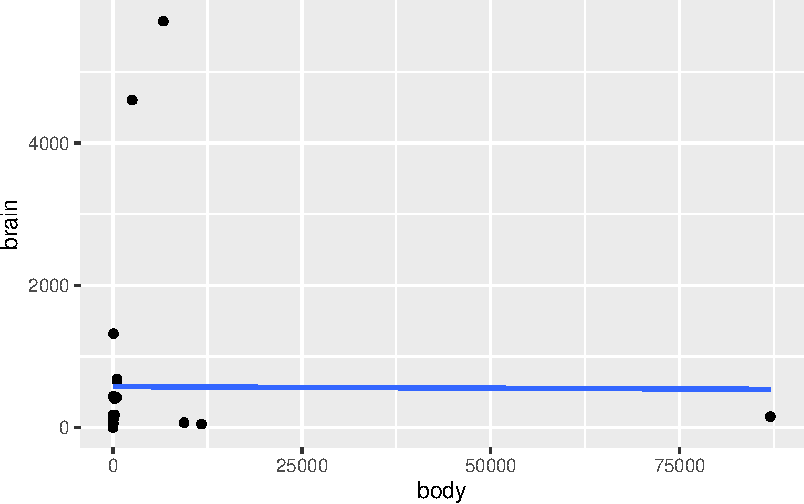
\includegraphics{stats_review_files/figure-pdf/unnamed-chunk-31-1.pdf}
\end{center}

Now that we plotted the data, however, we can clearly see that there is
an observation that is far to the right and is skewing the distribution
of \texttt{body}. Should we drop that observation to improve our
regression model or should we leave it there? Feel free to continue the
analysis with the tools you developed so far!

\subsubsection{Additional resources}\label{additional-resources-1}

Since it is impossible to discuss everything about regressions in these
few pages, here are some resources that you can find useful when trying
to make sense of this topic:

\begin{enumerate}
\def\labelenumi{\arabic{enumi}.}
\tightlist
\item
  \href{https://youtu.be/14mkCpJ7tKs?si=gF17WGfWBTTOf38z}{YT short intro
  to regression Video}
\item
  \href{https://youtube.com/playlist?list=PLblh5JKOoLUIzaEkCLIUxQFjPIlapw8nU&si=ldwNn7dwyE6ts7Q-}{YT
  Playlist on regression}
\item
  \href{https://www.youtube.com/@statquest}{Funny (but useful) Stats
  channel}
\end{enumerate}




\end{document}
